\documentclass[letterpaper,11pt,leqno]{article}
\usepackage{paper}
\usepackage{amsmath}
\usepackage{array}
\usepackage{float}
\usepackage{tabularx}
\usepackage{pdflscape}
\bibliographystyle{paper}

\title{The Sugar Paradox: National Food Supply Predicts Obesity across Countries but Not within Them}

\author{Blinded for review}

\date{}


\hypersetup{pdftitle={The Sugar Paradox: National Food Supply Predicts Obesity across Countries but Not within Them},pdfauthor={Blinded for review}}

\begin{document}

\begin{titlepage}
\maketitle

\noindent Countries that eat more sugar are fatter.
Across 37 Sub-Saharan African countries, national sugar supply predicts women's obesity at $r = 0.50$ after controlling for income, urbanization, and vegetable oil supply.
The association survives every cross-sectional stress test: leave-one-out exclusion, subregion fixed effects, rank correlations.

It does not survive following the same countries over time.
In a 2010--2022 panel, sugar supply is null within countries under six specifications---fixed effects, two-way fixed effects, detrending, first differences, long differences, and correlated random effects---each removing a different class of confounding, all converging on the same answer.
The null is not about sugar. None of 10 FAOSTAT food groups predicts within-country obesity change. A targeted grand-total energy, fat, and protein comparator reaches the same boundary under two-way fixed effects and first differences. Entity and year fixed effects absorb 99.4\% of obesity variance, leaving 0.6\% for any food variable to explain.

Standard safeguards do not catch this. A soybean oil case study passes cross-sectional tests, one-way fixed effects, and Oster bounds ($\delta = 17.6$), yet its lead-lag ratio is 0.99---pure co-trending with no temporal direction. The problem is global: 98\% of 200 countries show linear obesity trends ($R^2 \geq 0.90$).

The only predictor of which countries gained more obesity is how much they had to start with ($t = 3.45$). Cross-sectional associations between food supply and obesity---including those cited in support of sugar-sweetened beverage taxes---identify shared development trends, not dietary effects.

\end{titlepage}

% -----------------------------------------------
% 1. Introduction
% -----------------------------------------------
\section{Introduction}

Countries that consume more sugar are fatter. Plot national sugar supply against adult obesity prevalence for 37 Sub-Saharan African countries and the correlation is strong: $r = 0.50$ after controlling for GDP, urbanization, and vegetable oil supply ($p = 0.002$). Drop any single country and the result holds (leave-one-out range: 0.42--0.63). Add subregion fixed effects and the correlation strengthens to $r = 0.63$. By every conventional cross-sectional standard, sugar supply predicts obesity.

This paper shows that the association is entirely misleading. When we follow the same 37 countries over 13 years, tracking whether rising or falling sugar supply corresponds to faster or slower obesity growth, the association vanishes. Country fixed effects reduce the sugar coefficient to $t = 0.25$. Adding year effects drops it to $t = -0.64$. Detrending each country's individual trajectory gives $t = -0.13$. Three further approaches confirm the null: first differences ($r = -0.03$), long differences over the full decade ($r = -0.19$), and a Mundlak correlated random effects model ($t = -0.66$). Six specifications, each removing a different class of confounding, converge on the same answer: no signal.

The explanation is structural. Obesity has risen along near-linear trajectories in virtually every country over the past decade, and these trajectories have little to do with food supply. Entity and year fixed effects together absorb 99.4\% of obesity variance in our panel. Food supply variables compete for the remaining 0.6\%, a residual space dominated by measurement error and short-run noise. None of the 10 FAOSTAT food groups we test predicts within-country obesity. A targeted grand-total energy, fat, and protein comparator reaches the same boundary under two-way fixed effects and first differences. The null is not specific to sugar.

The mechanism is not subtle. Cross-sectional studies compare countries at a point in time, and such comparisons conflate persistent between-country differences with the shared upward trend in obesity. A correlated random effects decomposition confirms this: the between-country sugar coefficient is $t = 3.46$ while the within-country coefficient is $t = -0.66$. The entire association is between-country. A soybean oil case study makes the mechanism concrete. Soybean oil supply passes the same cross-sectional and one-way fixed-effects tests that sugar passes, yet its lead-lag ratio is 0.99: pure co-trending with no temporal direction.

The paradox matters because cross-sectional food supply studies have shaped policy. \citet{basu2013} applied generalized estimating equations to repeated cross-sections in 175 countries and argued that sugar availability independently predicted diabetes prevalence. A companion study \citep{basu2013ajph} linked soft drink consumption to overweight across 75 countries using purely cross-sectional regression, a finding cited over 500 times and invoked in WHO guidance on sugar-sweetened beverage taxation \citep{who2023ssb}. Both studies draw their identification from between-country variation, exactly the variation we show is confounded by shared trends. More broadly, the Global Burden of Disease project assigns diet-attributable deaths using food supply data that faces the same trend-domination problem \citep{gbd2019}, and a recent global analysis attributed 2.2 million new diabetes cases to sugar-sweetened beverages using dietary intake estimates informed in part by national food supply data \citep{laracastor2025}. Any study that relies on cross-national food supply variation to identify dietary effects inherits the confounding structure we document.

The problem is not specific to Sub-Saharan Africa. Among 200 countries in the NCD-RisC database \citep{ncdrisc2024bmi}, 98\% show linear obesity trends with $R^2 \geq 0.90$ over 2010--2021. This near-universal linearity means that any food supply variable trending over the same period will correlate with obesity cross-sectionally, regardless of whether it causes obesity.

If food supply changes do not predict obesity change, what does? The only predictor is initial obesity level ($t = 3.45$, $R^2 = 0.41$). Countries that started with higher obesity in 2010 gained more over the following decade. This divergence pattern points to structural economic and demographic conditions rather than dietary composition as the driver of cross-country obesity differences.

The paper proceeds as follows. Section 2 describes the data. Section 3 documents the paradox. Section 4 diagnoses why it exists. Section 5 shows the problem is global and revisits published results. Section 6 examines what does predict obesity change. Section 7 discusses implications.

% -----------------------------------------------
% 2. Data and Panel Construction
% -----------------------------------------------
\section{Data and Panel Construction}

\subsection{Sources}

We construct a country-year-sex panel for 37 Sub-Saharan African countries from 2010 through 2022, combining three data sources.

\paragraph{Food supply} FAOSTAT Food Balance Sheets \citep{faostat2024} provide national food supply in kilocalories per capita per day for 10 food groups: cereals, sugar \& sweeteners, vegetable oils, meat, milk, fruits, vegetables, starchy roots, pulses, and animal fats. The primary exposure variable is sugar \& sweeteners supply (mean 164 kcal/cap/day, SD 107). We also examine vegetable oils (mean 233, SD 108) and all remaining food groups in robustness analyses. For the aggregate-energy comparator, we extract FAOSTAT grand-total energy, fat, and protein supply from the same release. Soybean oil supply, used in the case study of Section 4, also comes from this release.

\paragraph{Health outcomes} NCD-RisC Lancet 2024 estimates \citep{ncdrisc2024bmi} provide age-standardized adult obesity prevalence (BMI $\geq$ 30) for each country-year-sex cell. Women's mean obesity prevalence is 17.1\% (SD 10.0); men's is 6.2\%. We also examine diabetes prevalence from the companion NCD-RisC release \citep{ncdrisc2024diabetes} (women's mean 10.1\%, men's 9.2\%). These estimates come from a Bayesian hierarchical model that pools population-representative surveys, producing smooth temporal trajectories that we return to in Section 4.

\paragraph{Covariates} GDP per capita in constant 2015 US dollars (mean \$2,429, SD \$3,088) and urban population share (mean 43.5\%, SD 16.9) come from the World Development Indicators \citep{wdi2024}.

\subsection{Panel Structure}

The panel contains 962 observations: 37 countries $\times$ 13 years $\times$ 2 sexes, with no missing cells. All obesity and diabetes values validate exactly against the raw NCD-RisC files (zero mismatches across 962 checked values). The 37-country boundary is structural: 11 SSA countries are absent from the comparable FAOSTAT Food Balances (2010--) release and cannot be recovered without breaking cross-country comparability. This boundary is a design restriction, not a data-repair problem.

\subsection{Cross-Sectional Specification}

Analyses that require a single cross-section (partial correlations, leave-one-out tests, subregion comparisons) average each variable over 2018--2020 to reduce year-specific noise while staying within the panel period. All cross-sectional analyses throughout the paper use this same time window for internal consistency.

\subsection{Descriptive Summary}

Table~\ref{tab:descriptives} reports summary statistics for the women's panel ($N = 481$). All within-country regression results reported in subsequent sections use women's data unless otherwise noted.

\begin{table}[htbp]
\caption{Summary statistics for the 37-country, 2010--2022 analysis panel (women only, $N = 481$).}
\label{tab:descriptives}
\begin{tabular*}{\textwidth}{@{\extracolsep\fill}lrrrrr}
\toprule
Variable & $N$ & Mean & SD & Min & Max \\
\midrule
Obesity prevalence (\%) & 481 & 17.09 & 9.96 & 2.12 & 47.35 \\
Diabetes prevalence (\%) & 481 & 10.12 & 3.87 & 4.21 & 25.57 \\
Sugar supply (kcal/cap/day) & 481 & 163.76 & 107.46 & 20.49 & 526.78 \\
Vegetable oils (kcal/cap/day) & 481 & 233.26 & 107.85 & 16.27 & 564.16 \\
GDP per capita (2015 USD) & 481 & 2,429 & 3,088 & 401 & 19,482 \\
Urban population (\%) & 481 & 43.54 & 16.90 & 15.48 & 91.22 \\
\bottomrule
\end{tabular*}
\end{table}

For the global analysis of Section 5, we use the full NCD-RisC database covering 200 countries (2010--2021) without restricting to FAOSTAT availability.

% -----------------------------------------------
% 3. The Paradox Documented
% -----------------------------------------------
\section{The Paradox Documented}

\subsection{Cross-Sectional Evidence}

Sugar supply predicts obesity across countries. Using 2018--2020 country means for women, the bivariate correlation between sugar supply and obesity prevalence is $r = 0.68$ ($p < 0.001$, $N = 37$). Controlling for GDP per capita, urbanization, and vegetable oil supply, the partial correlation remains $r = 0.50$ ($p = 0.002$). Figure~\ref{fig:cross_sectional} shows both relationships.

The association is robust to standard cross-sectional stress tests. Leave-one-out analysis yields partial correlations ranging from 0.42 (dropping Mauritania) to 0.63 (dropping Gambia), with no single country driving the result. Adding subregion fixed effects strengthens the partial correlation to $r = 0.63$ ($p < 0.001$). Adding both subregion and GDP controls gives $r = 0.46$ ($p = 0.004$). Replacing Pearson with Spearman rank correlations preserves the pattern. By every conventional cross-sectional criterion, sugar supply is a strong, stable predictor of obesity.

\begin{figure}[htbp]
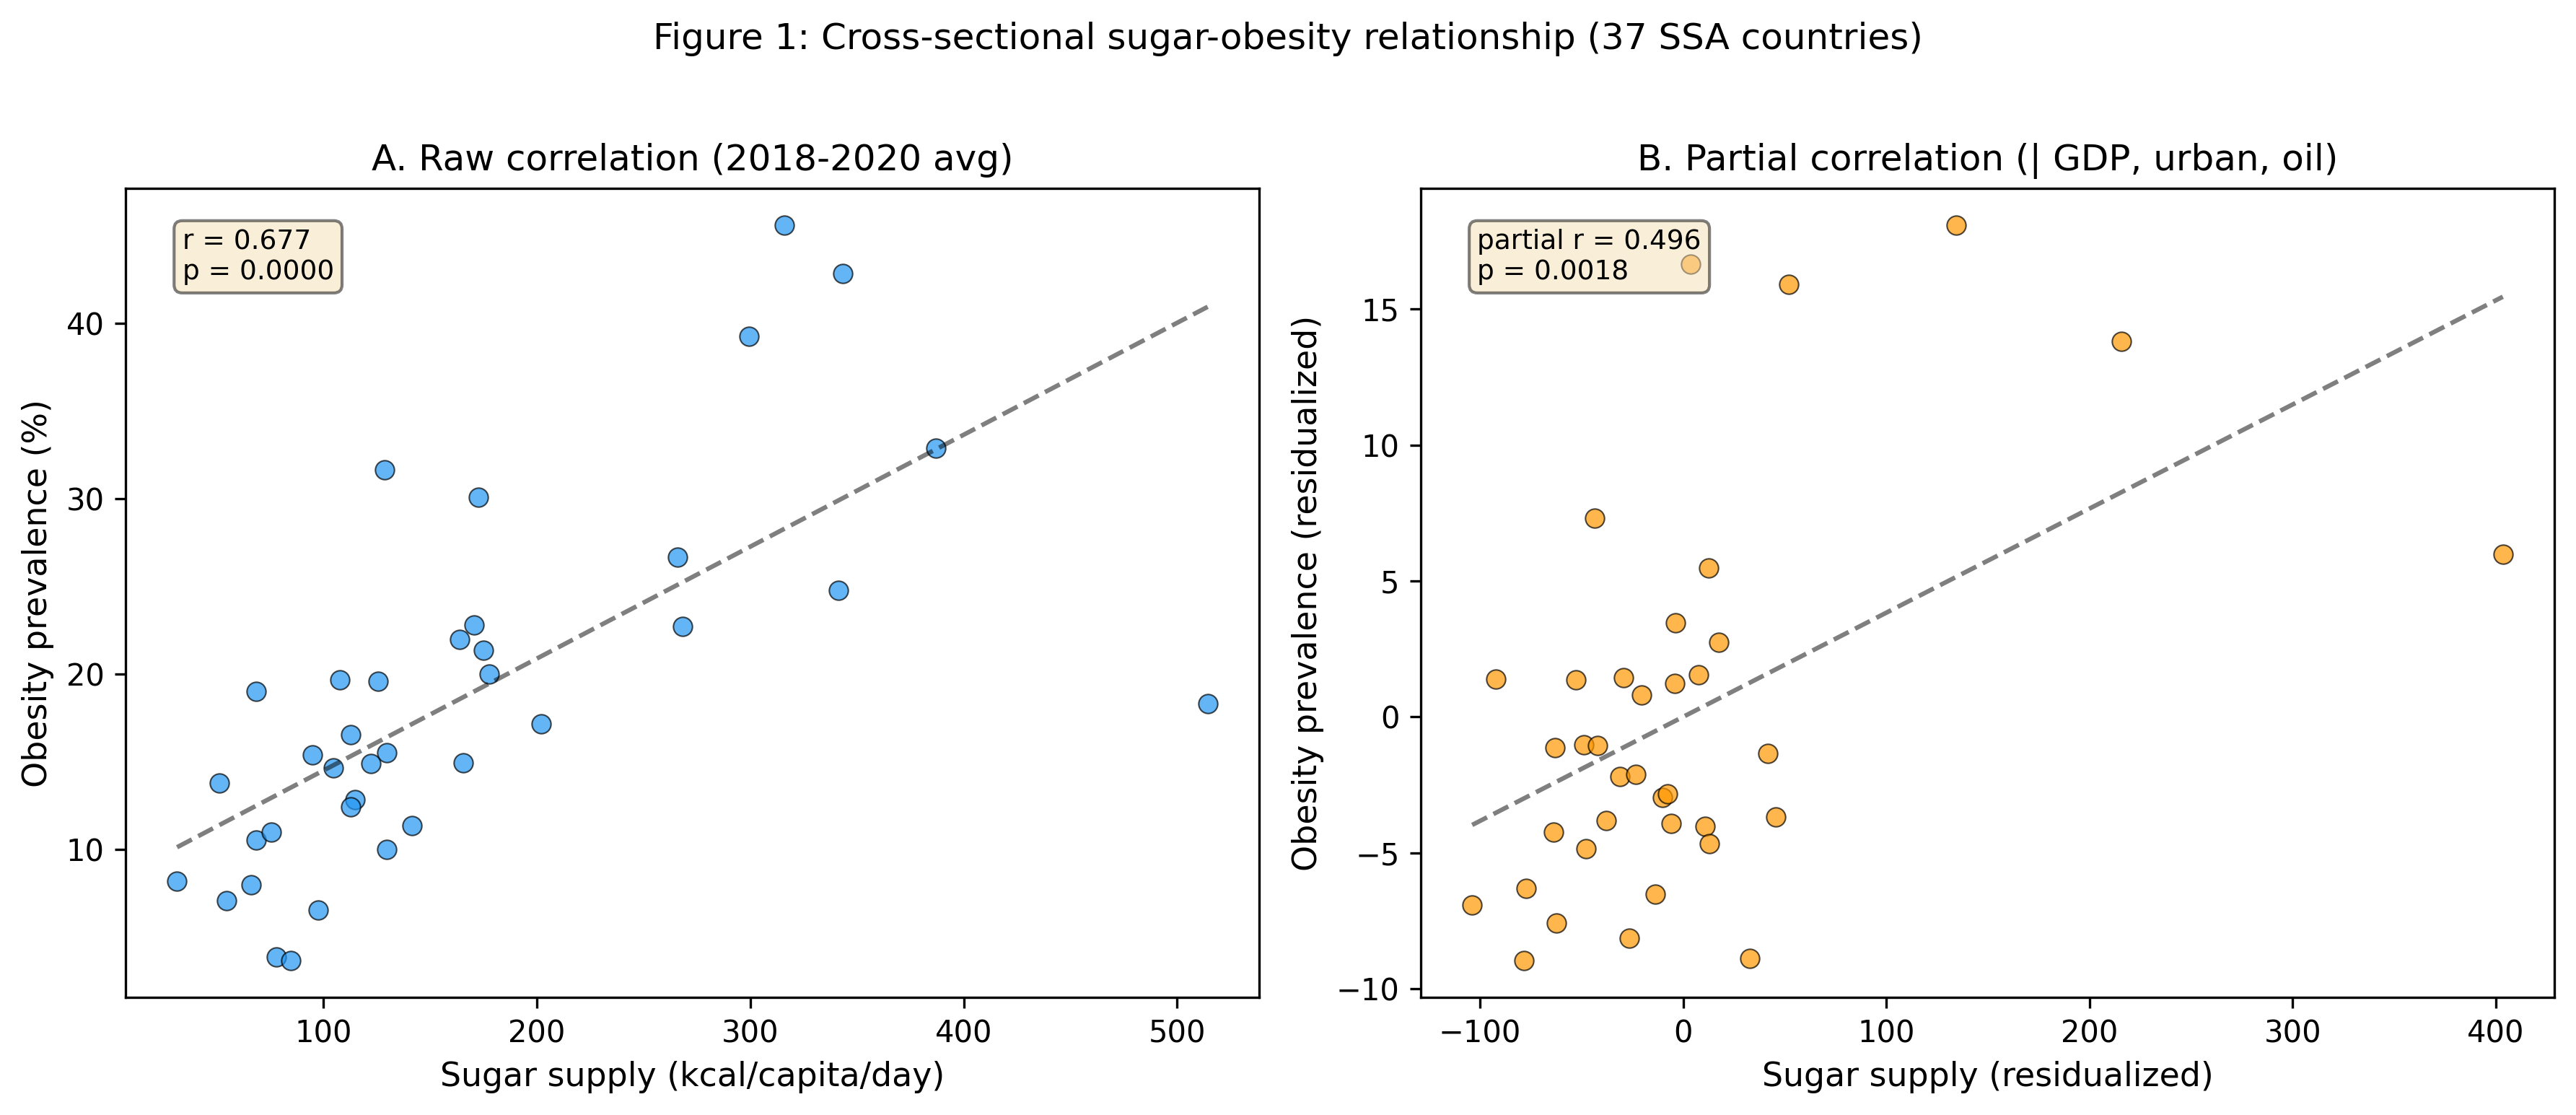
\includegraphics[width=\textwidth]{../../figures/fig1_cross_sectional.png}
\caption{Cross-sectional association between sugar supply and women's obesity, 2018--2020 country means. Left: bivariate ($r = 0.68$). Right: partial correlation after controlling for GDP, urbanization, and vegetable oil supply ($r = 0.50$, $p = 0.002$).}
\label{fig:cross_sectional}
\end{figure}

\subsection{Within-Country Evidence}

The cross-sectional association vanishes when we follow the same countries over time. Table~\ref{tab:fe_cascade} reports the sugar coefficient under progressively demanding specifications, all with standard errors clustered at the country level \citep{bertrand2004}.

\begin{table}[htbp]
\caption{Sugar supply coefficient across specifications, controlling for vegetable oil supply. Dependent variable: women's obesity prevalence (\%). Standard errors clustered by country for FE specifications ($N_{\text{clusters}} = 37$, $N_{\text{obs}} = 481$).}
\label{tab:fe_cascade}
\begin{tabular*}{\textwidth}{@{\extracolsep\fill}lccccc}
\toprule
Specification & $\hat{\beta}_{\text{sugar}}$ & SE & $t$ & $p$ & $R^2$ \\
\midrule
Pooled OLS & 0.630 & 0.032 & 19.84 & $< 0.001$ & 0.49 \\
Country FE & 0.035 & 0.136 & 0.25 & 0.80 & 0.96 \\
Two-way FE & $-0.029$ & 0.045 & $-0.64$ & 0.52 & 0.99 \\
Detrended & $-0.001$ & 0.006 & $-0.13$ & 0.90 & 0.01 \\
\bottomrule
\end{tabular*}
\end{table}

Pooled OLS, which mixes between-country and within-country variation, yields a strong sugar coefficient ($t = 19.84$). Adding country fixed effects absorbs the between-country signal and the coefficient drops to $t = 0.25$. Adding year fixed effects drops it further to $t = -0.64$. Entity-specific linear detrending, which removes each country's individual trajectory, yields $t = -0.13$.

Wild-cluster bootstrap $p$-values match the asymptotic clustered results: $p = 0.80$ for country fixed effects and $p = 0.58$ for two-way fixed effects (999 bootstrap draws). A permutation test that shuffles within-country sugar ordering yields $p = 0.58$. Two-way clustering by country and year gives $t = -0.63$, identical to one-way clustering. The null does not depend on the choice of standard error.

Three additional specifications confirm the null. First differences correlate annual changes in sugar with annual changes in obesity: $r = -0.03$ ($p = 0.59$, $N = 444$). Long differences, comparing only the 2010 and 2020 endpoints, yield $r = -0.19$ ($p = 0.25$, $N = 37$). Because long differences do not depend on year-to-year variation, they resist the NCD-RisC smoothing discussed in Section 4.

A Mundlak correlated random effects model \citep{mundlak1978} makes the between-within decomposition explicit. The model includes both time-varying sugar supply and its country mean as regressors, so the coefficients on each cleanly estimate within-country and between-country associations. The within-country sugar coefficient is $t = -0.66$; the between-country coefficient is $t = 3.46$. The entire cross-sectional association comes from between-country variation. Within countries, sugar supply and obesity are unrelated.

Figure~\ref{fig:fe_cascade} visualizes the specification cascade.

\begin{figure}[htbp]
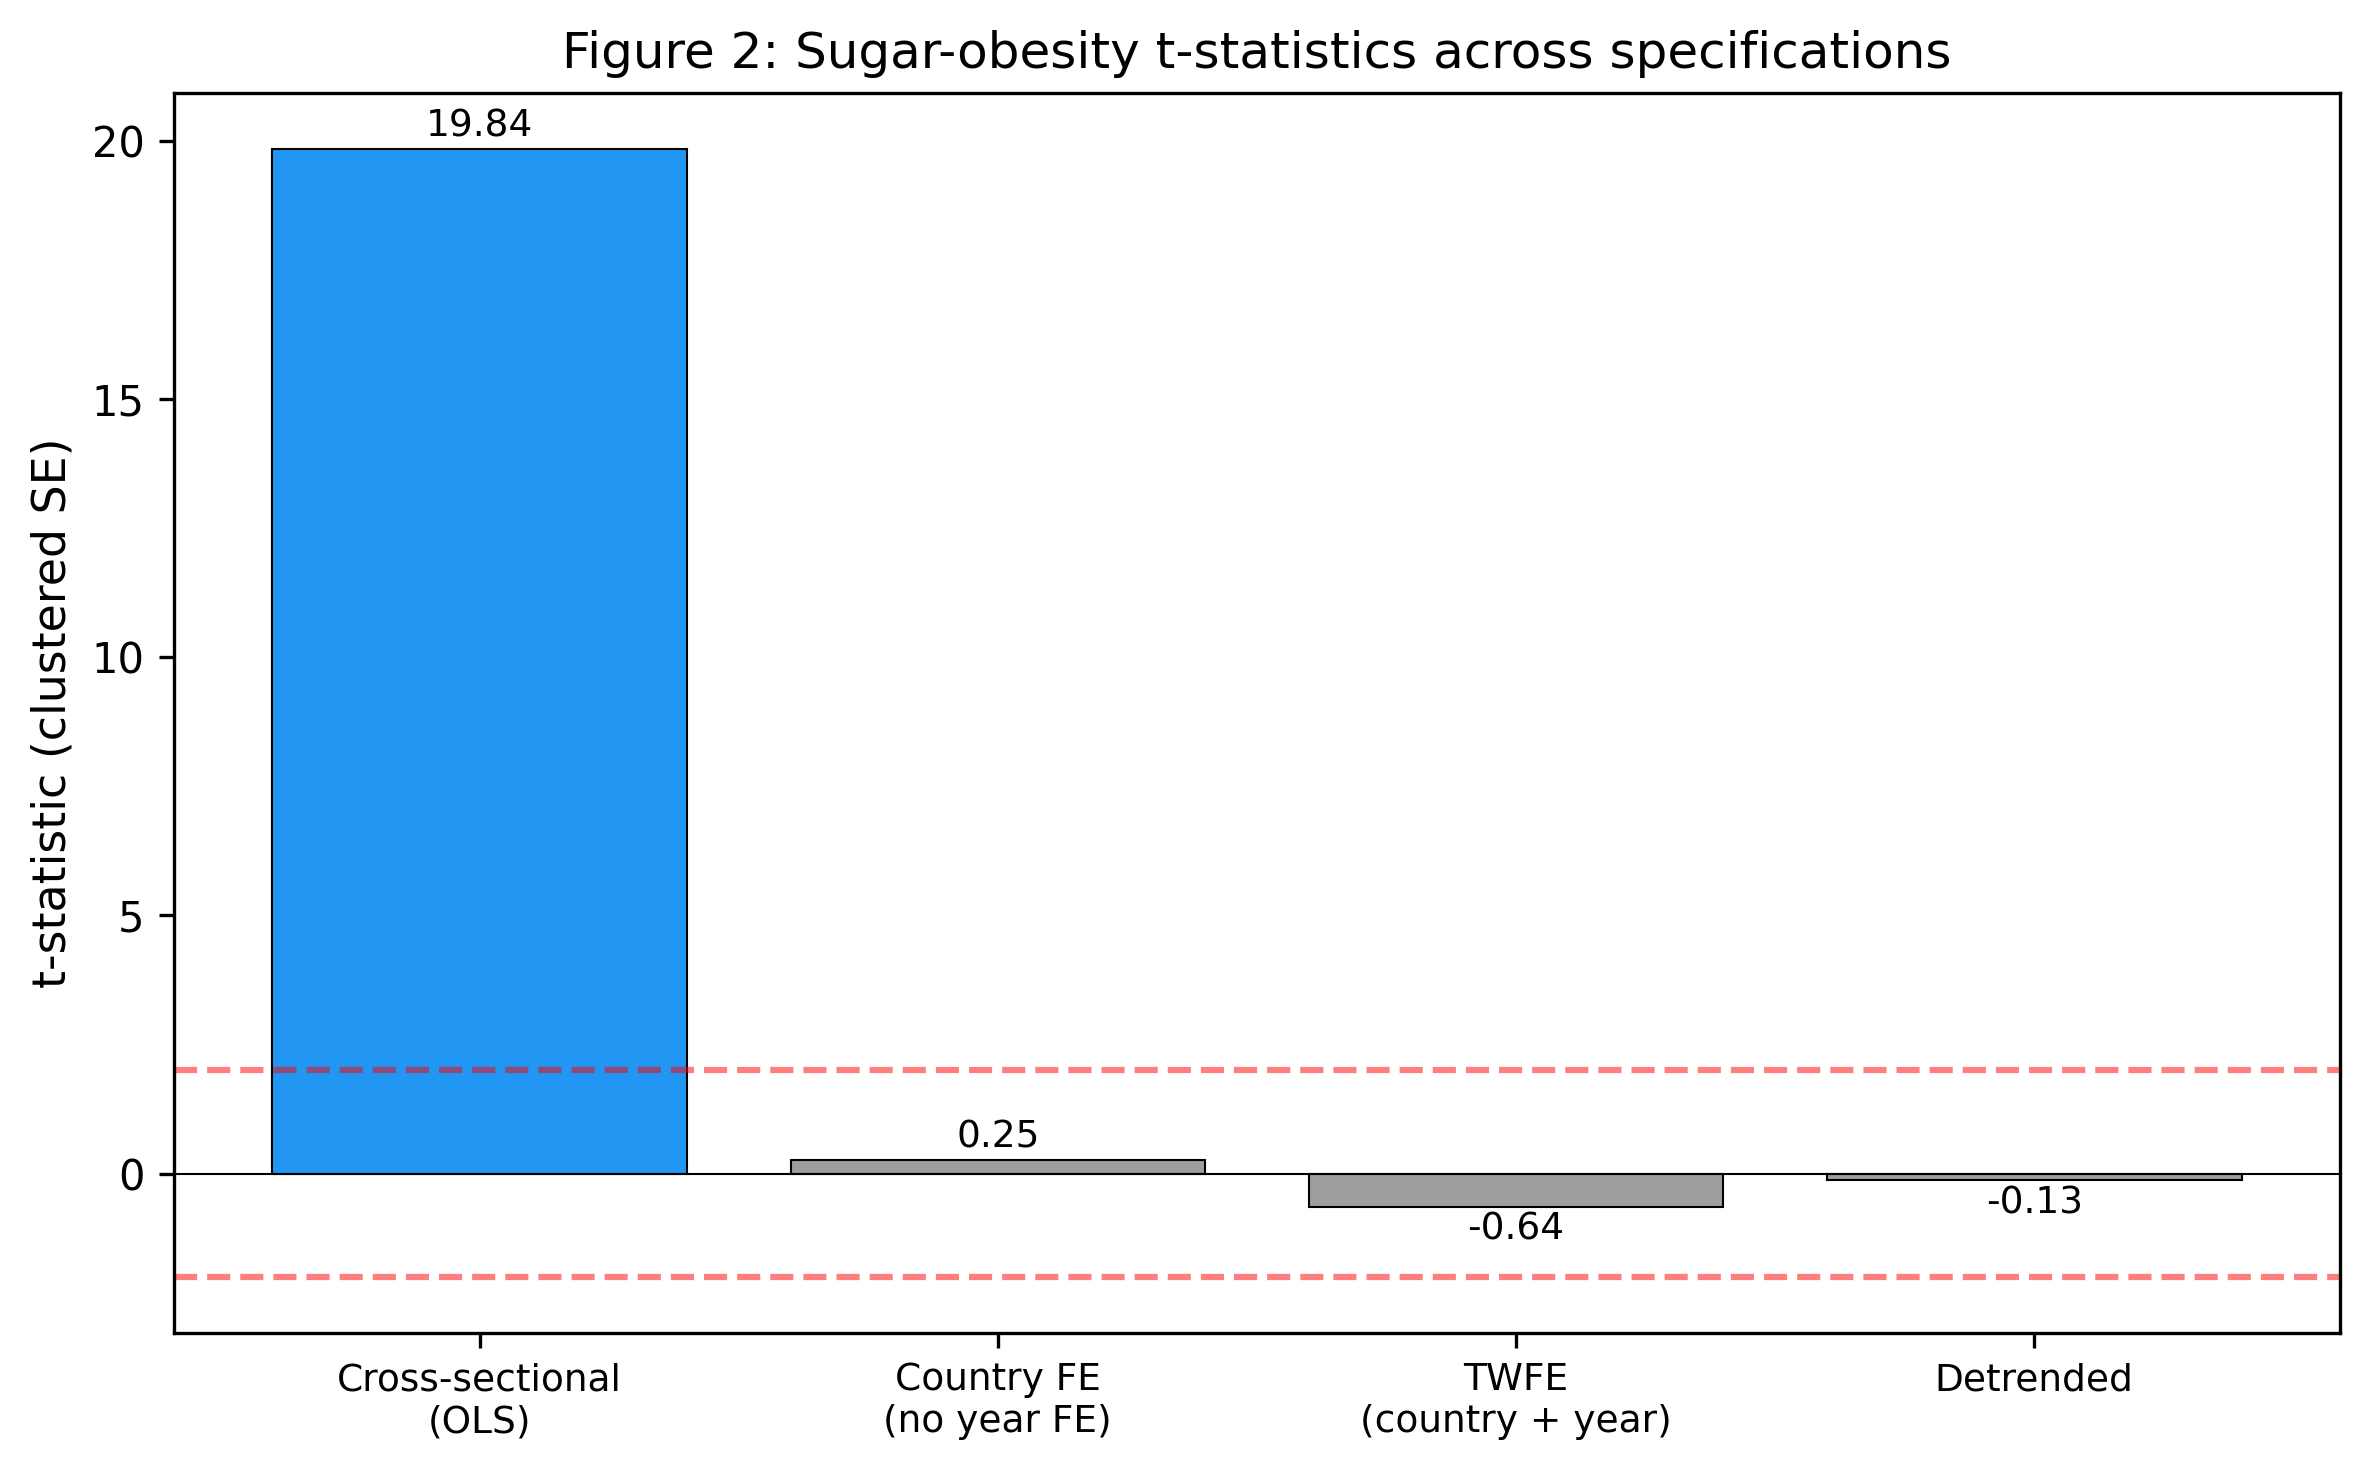
\includegraphics[width=\textwidth]{../../figures/fig2_fe_cascade.png}
\caption{Sugar supply coefficient under progressively demanding specifications. The coefficient drops from strongly positive (pooled OLS) to null once within-country variation is isolated.}
\label{fig:fe_cascade}
\end{figure}

\subsection{Generality Beyond Sugar}

The null is not specific to sugar. We tested all 10 FAOSTAT food groups under four specifications: cross-sectional correlation, one-way country fixed effects, two-way fixed effects, and first differences. Six of 10 food groups show significant cross-sectional associations with obesity. Two of 10 remain significant under one-way country fixed effects (meat at $t = 3.05$ and vegetables at $t = 4.13$). Zero of 10 survive two-way fixed effects. Zero of 10 survive first differences. Sugar, meat, milk, and several other food groups look strong in cross-country comparisons, but that signal disappears once shared trends are removed. In this panel, no food-supply variable shows a stable within-country association with obesity.

Recent FAOSTAT-based obesity studies emphasize aggregate energy and nutrient supply rather than individual food groups \citep{siminiuc2025,delgadopertinez2026}. We therefore ran a targeted comparator on grand-total energy, fat, and protein supply. Table~\ref{tab:energy_comparator} shows the same boundary. Total energy is null under two-way fixed effects ($t = -1.32$, $p = 0.19$) and remains null after adding GDP and urban controls ($t = -1.03$, $p = 0.30$). First differences are also null ($t = -0.57$, $p = 0.57$). Fat and protein are null across the same checks. A simple country-linear detrended energy residual is positive ($t = 2.98$, $p = 0.003$). But it weakens after adding year fixed effects ($t = 1.74$, $p = 0.08$), and both lagged and lead energy residuals carry signal (lag $t = 2.98$, lead $t = 2.19$). That pattern is residual co-movement, not directional evidence that national energy supply explains obesity change.

\begin{table}[htbp]
\centering
\caption{Grand-total FAOSTAT comparator against total energy and macronutrients. Entries are country-clustered $t$-statistics for women's obesity prevalence. TWFE + controls includes GDP per capita and urban population share.}
\label{tab:energy_comparator}
\small
\begin{tabular}{lrrrr}
\toprule
Feature & TWFE & TWFE + controls & Detrended & First diff. \\
\midrule
Total energy (+100 kcal/cap/day) & $-1.32$ & $-1.03$ & $2.98^{**}$ & $-0.57$ \\
Total fat (+10 g/cap/day) & $-1.59$ & $-1.44$ & $-0.64$ & $-0.99$ \\
Total protein (+10 g/cap/day) & $-0.78$ & $-0.18$ & $1.50$ & $-0.18$ \\
\bottomrule
\multicolumn{5}{l}{\footnotesize $^{**}p < 0.01$. Detrended removes a country-specific linear trend only.}
\end{tabular}
\end{table}

This uniformity points to a structural explanation. Entity and year fixed effects absorb 99.4\% of obesity variance. The residual 0.6\% is too small and too noisy for any food supply variable to predict, regardless of whether that variable has a genuine causal relationship with obesity at the individual level.

\subsection{Diabetes: The Borderline Case}

Diabetes is the one outcome where the within-country sugar signal approaches significance. Under two-way fixed effects, the women's diabetes sugar coefficient is $t = 1.92$ ($p = 0.055$). A Mundlak decomposition gives a within-country coefficient of $t = 1.99$. This is the closest any specification gets to a conventional threshold in the entire analysis.

The explanation is structural. Entity and year fixed effects absorb 95.6\% of diabetes variance, compared to 99.4\% for obesity. That leaves 4.4\% residual variance---7.7 times more room for food supply variables to find something. The borderline TWFE coefficient exploits this extra room. But entity-specific linear detrending, which removes each country's individual diabetes trajectory, yields $t = 0.26$ ($p = 0.80$). First differences yield $r = 0.04$ ($p = 0.41$). Long differences yield $r = 0.24$ ($p = 0.15$). The TWFE signal is residual co-trending that detrending kills. Diabetes shows the same paradox as obesity, with more noise in the residual.

\subsection{GBD Dietary Intake Variables}

In exploratory analysis of 15 dietary intake variables from the Global Burden of Disease 2021 study (fruits, vegetables, legumes, whole grains, nuts, red meat, processed meat, sugar-sweetened beverages, sodium, fiber, calcium, omega-3, polyunsaturated fat, trans fat, and milk), the same pattern held: cross-sectional correlations collapsed under fixed effects. These GBD estimates combine survey data with food supply proxies \citep{gbd2019}, so they are not independent of the FAOSTAT measurement issues we discuss in Section 7. The pattern is consistent with the structural explanation, though we present the GBD results as suggestive rather than definitive.

% -----------------------------------------------
% 4. Diagnosis
% -----------------------------------------------
\section{Diagnosis}

The cross-sectional association is too strong and too stable to be noise, yet within-country evidence is too consistently null to be a power problem. This section diagnoses four structural features of the data that produce the paradox, then illustrates all four with a case study.

\subsection{Trend Domination}

Obesity trends in SSA are near-linear and account for almost all variation. Within each country, the mean linear trend $R^2$ is 0.995. A pooled regression of women's obesity on country indicators and a common linear time trend yields $R^2 = 99.4\%$. These trends persist in countries where sugar supply rose, fell, or remained flat. Food supply does not explain them. The result is the spurious regression problem identified by \citet{granger1974} in time series and extended to panel data by \citet{kao1999}: trending series correlate mechanically, regardless of causal connection.

Entity fixed effects alone absorb 95.7\% of obesity variance by removing between-country level differences. Year fixed effects absorb an additional 3.7\%, capturing the shared upward trend. Together they explain 99.4\%, leaving 0.6\% for any food supply variable to predict. This residual is tiny, dominated by measurement error and short-run deviations from trend.

Figure~\ref{fig:variance_decomp} shows the decomposition.

\begin{figure}[htbp]
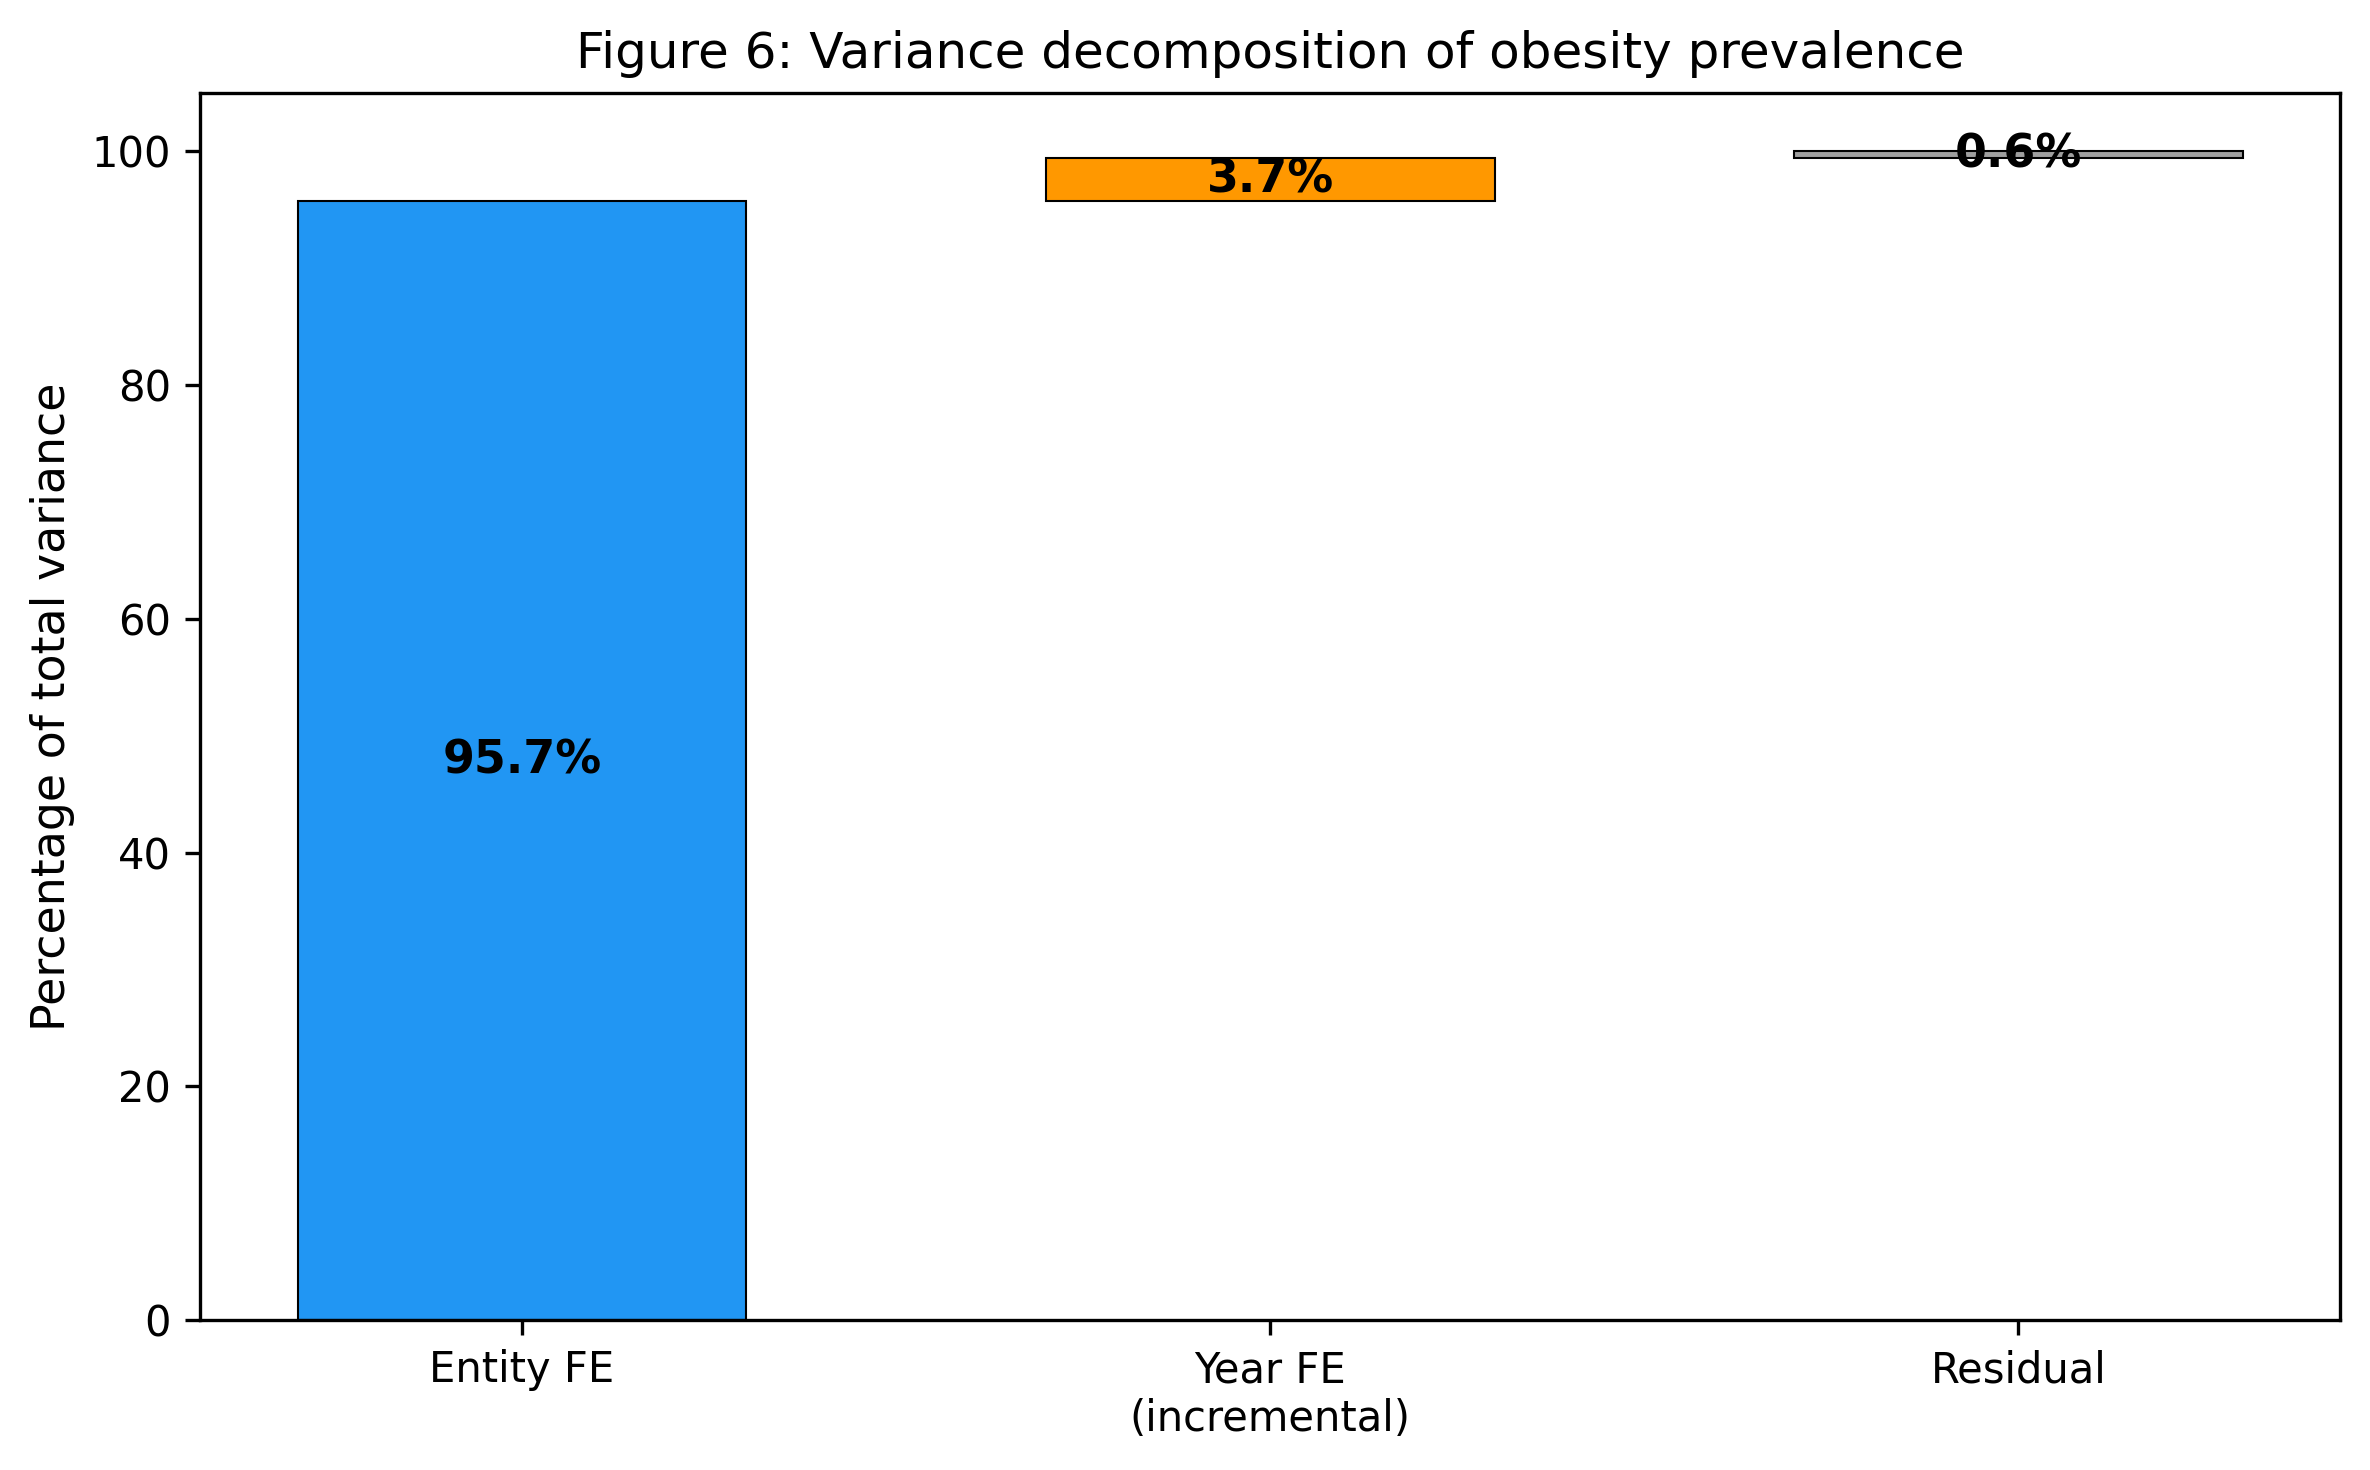
\includegraphics[width=0.7\textwidth]{../../figures/fig6_variance_decomposition.png}
\caption{Variance decomposition of women's obesity prevalence. Entity fixed effects absorb 95.7\% and year fixed effects 3.7\%. Food supply variables compete in the remaining 0.6\%.}
\label{fig:variance_decomp}
\end{figure}

The near-linear trend has a second consequence for cross-sectional inference. Comparisons across countries at a point in time conflate two sources of variation: persistent between-country differences (which drive the level ordering) and the shared upward trend (which widens the gaps over time). Countries with higher sugar supply also tend to be more economically developed, more urbanized, and further along the nutrition transition \citep{popkin2012}. These characteristics independently predict obesity through level differences that fixed effects absorb.

\subsection{Standard Error Inflation}

Country-level clustering inflates standard errors by a factor of 2.6$\times$ to 2.9$\times$ across sugar specifications. Without clustering, the one-way FE sugar coefficient has $t = 0.73$; with clustering, $t = 0.25$. The inflation arises because within-country observations are serially correlated: the mean first-order autocorrelation of panel residuals is 0.90. Non-clustered standard errors treat these correlated observations as independent, inflating t-statistics by a factor of roughly three.

This inflation matters because published studies that report non-clustered standard errors in country-level panels will overstate significance by the same factor. A coefficient that appears significant at $t = 2.0$ with non-clustered errors would require $t = 5$ to $6$ to survive clustering. \citet{bertrand2004} demonstrated this problem two decades ago for differences-in-differences designs, and \citet{abadie2023} formalized when clustering adjustments are necessary. The problem applies with equal force to country-level food supply panels. Standard error inflation does not explain the paradox (the coefficient itself is null), but it explains how weak signals can appear significant in models with insufficient clustering.

\subsection{NCD-RisC Smoothing}

The NCD-RisC obesity estimates come from a Bayesian hierarchical model that pools population-representative surveys \citep{ncdrisc2024bmi}. The model imposes smooth temporal trajectories and partial pooling across countries and regions.

This smoothing has two consequences. First, it compresses within-country variation. Annual deviations from trend are smaller in the NCD-RisC estimates than they would be in raw survey data, reducing the signal available for within-country regression. Second, partial pooling means each country's estimate borrows information from regional neighbors, potentially introducing spatial correlation absent from the underlying data.

We note this as a limitation rather than a correction. NCD-RisC data are the standard outcome measure in global obesity research; any finding using these data faces the same constraint. The relevant question is whether our null reflects genuine absence of association or insufficient variation after smoothing. The consistency of the null across six specifications argues for the former. Long differences, which compare only the 2010 and 2020 endpoints and do not depend on year-to-year variation, yield $r = -0.19$ (null). If sugar supply had a real within-country effect large enough to matter for policy, it should survive at least one of these approaches.

\subsection{The Soybean Oil Case Study}

Soybean oil supply provides a clean demonstration of how co-trending generates the paradox. No one would argue that soybean oil supply causes obesity in Sub-Saharan Africa, yet the variable passes the same tests sugar passes. Table~\ref{tab:soybean} reports eight diagnostic tests.

\begin{table}[htbp]
\caption{Soybean oil case study: diagnostic test battery. The variable passes cross-sectional and one-way FE tests but fails every trend-removal diagnostic, consistent with pure co-trending.}
\label{tab:soybean}
\begin{tabular*}{\textwidth}{@{\extracolsep\fill}lrl}
\toprule
Test & Statistic & Verdict \\
\midrule
Cross-sectional $r$ & 0.362 & significant ($p = 0.028$) \\
Country FE $t_{\text{cl}}$ & 2.09 & significant \\
Two-way FE $t_{\text{cl}}$ & 0.70 & null \\
Lead-lag ratio & 0.99 & co-trending \\
Detrended $t_{\text{cl}}$ & 1.62 & null \\
First differences $r$ & 0.035 & null \\
Granger $r$ & 0.053 & null \\
Oster $\delta$ & 17.6 & misleading \\
\bottomrule
\end{tabular*}
\end{table}

Soybean oil passes the two tests most commonly used in the literature. Cross-sectionally, $r = 0.36$ ($p = 0.028$). Under one-way country fixed effects, $t_{\text{cl}} = 2.09$. A researcher using these two approaches would conclude that soybean oil supply predicts obesity.

Six tests tell a different story. Two-way fixed effects reduce the coefficient to null ($t_{\text{cl}} = 0.70$). The lead-lag ratio, comparing coefficients on lead and lag of soybean oil, is 0.99. A causal variable would produce a lead coefficient smaller than the lag (the cause precedes the effect); a ratio near 1.0 indicates pure co-trending with no temporal direction. Detrending yields $t_{\text{cl}} = 1.62$ (null). First differences yield $r = 0.035$ (null). Granger causality yields $r = 0.053$ (null).

The Oster bounds $\delta$ illustrates a separate failure mode. \citeauthor{oster2019}'s method \citep{oster2019} asks how large unobserved confounding would need to be, relative to observed confounding, to explain away a coefficient. Soybean oil's $\delta = 17.6$ would normally indicate strong robustness to confounding. Here it is misleading: the $R^2$ jump from bivariate (0.12) to country FE (0.96) comes from fixed effects absorbing level differences, not from soybean oil genuinely predicting obesity. The $\delta$ is high because the wrong variation is being compared.

The case study matters because it is not an analogy. Soybean oil passes the same tests sugar passes: significant cross-sectional correlation, significant one-way FE, large Oster $\delta$. The tests that distinguish co-trending from causation (two-way FE, detrending, first differences, lead-lag, Granger) all reject. Standard approaches to food-supply-obesity association cannot distinguish co-trending from causal relationships.

\begin{figure}[htbp]
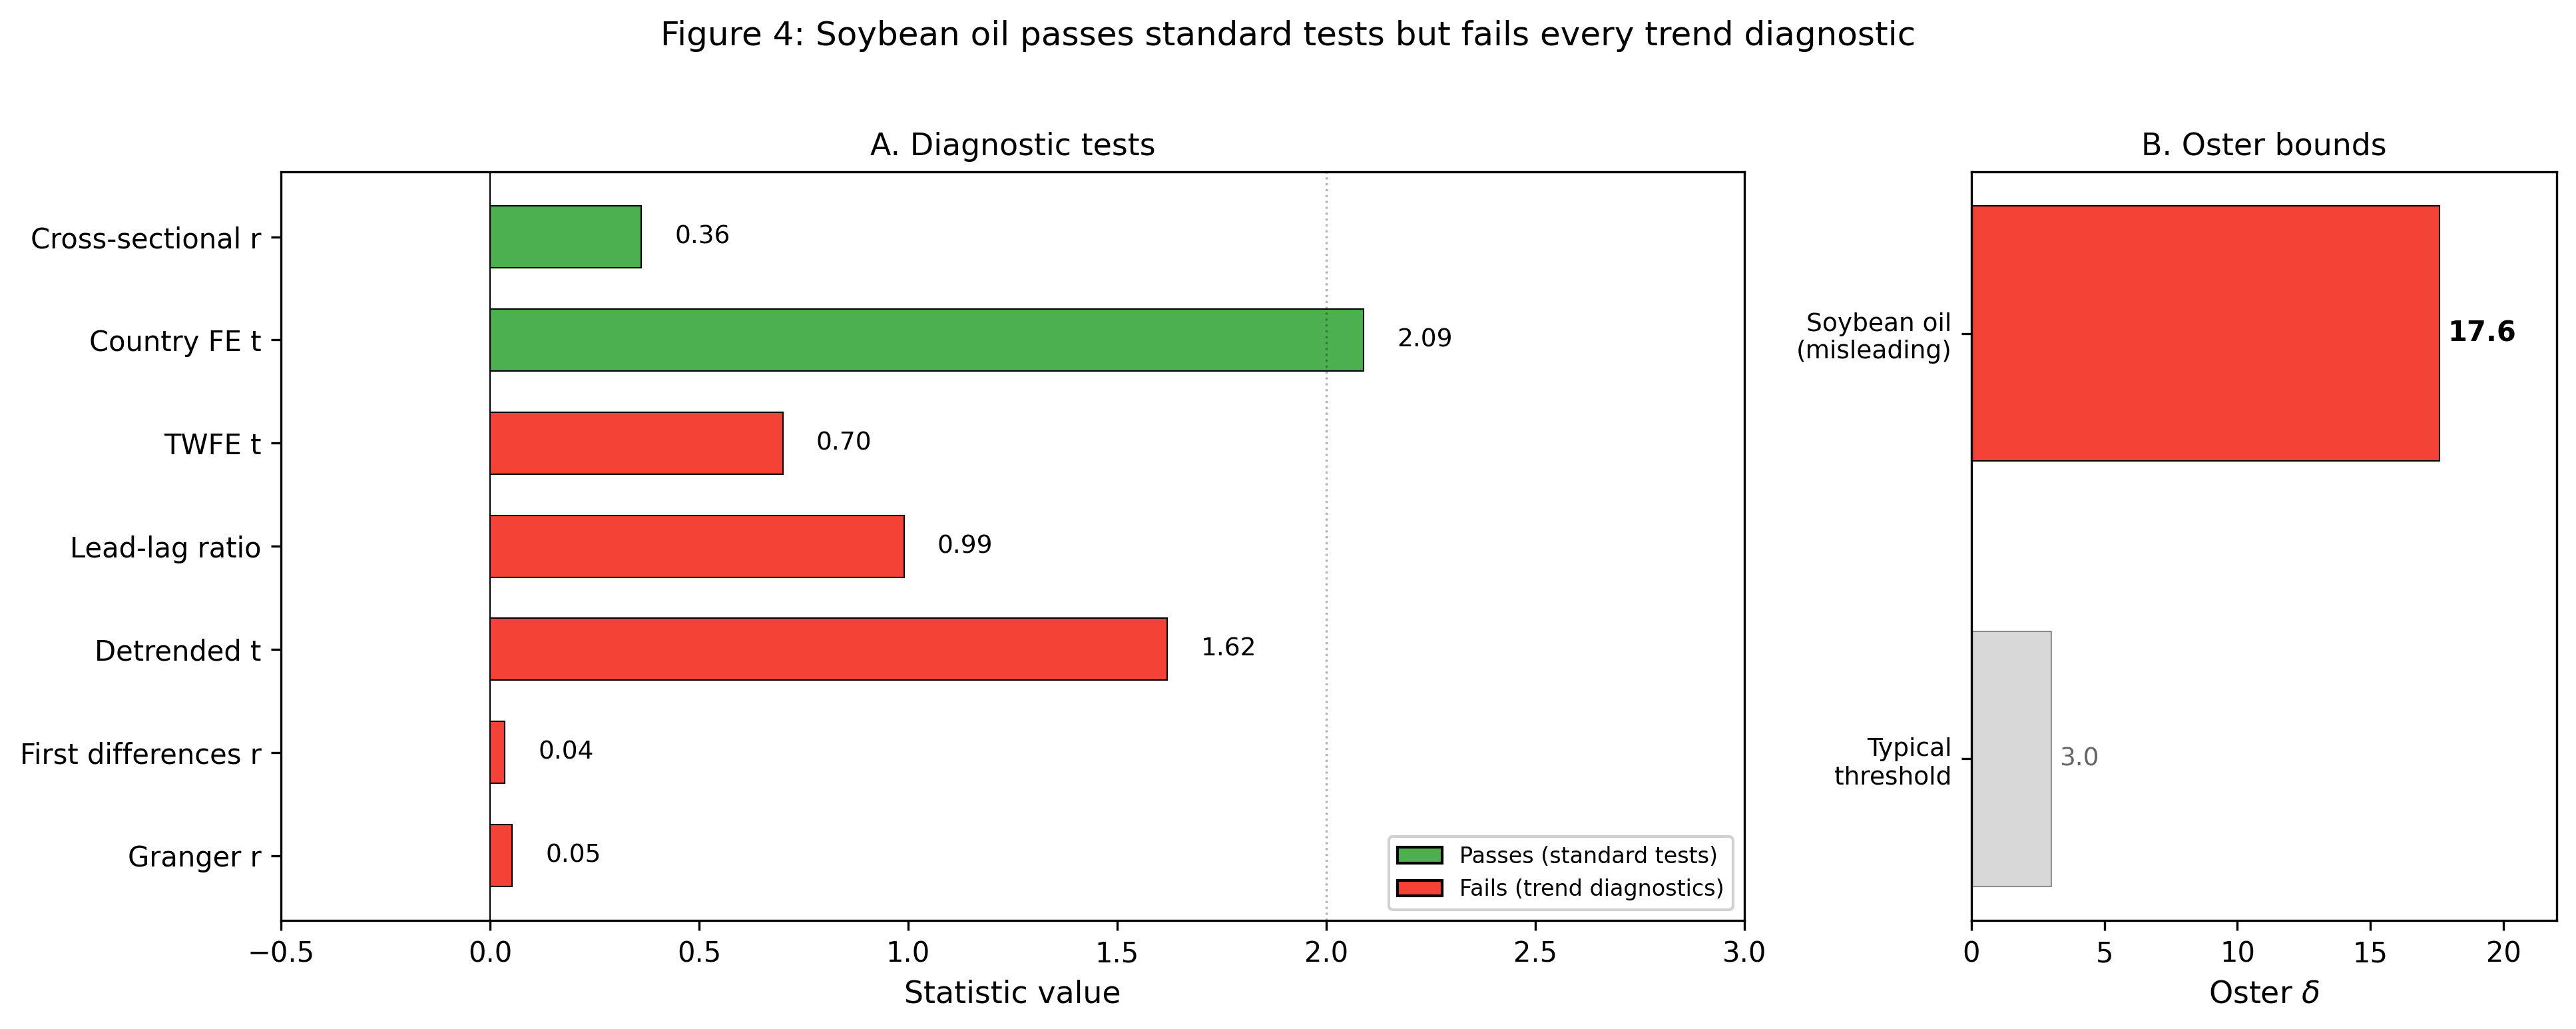
\includegraphics[width=\textwidth]{../../figures/fig4_soybean_oil_case.png}
\caption{Soybean oil case study: standard tests vs.\ trend diagnostics. The variable passes cross-sectional ($r = 0.36$) and one-way FE ($t_{\text{cl}} = 2.09$) tests but fails every trend-removal diagnostic. Lead-lag ratio of 0.99 confirms pure co-trending. Oster $\delta = 17.6$ is misleading (see text).}
\label{fig:soybean}
\end{figure}

% -----------------------------------------------
% 5. The Problem Is Global and Affects Published Results
% -----------------------------------------------
\section{The Problem Is Global and Affects Published Results}

\subsection{Global Scope of Trend Domination}

The paradox documented in Sections 3--4 uses 37 Sub-Saharan African countries. Is trend domination specific to this region? We test this by fitting country-specific linear trends to women's obesity prevalence for all 200 countries in the NCD-RisC database (2010--2021).

Of 200 countries, 196 (98.0\%) have linear trend $R^2 \geq 0.90$. The median is 0.999; the mean is 0.988. Only four countries fall below 0.90: Switzerland (0.03, a plateau), Venezuela (0.80, an economic crisis), Austria (0.83), and Lithuania (0.86). Figure~\ref{fig:global_trend} shows the distribution.

\begin{figure}[htbp]
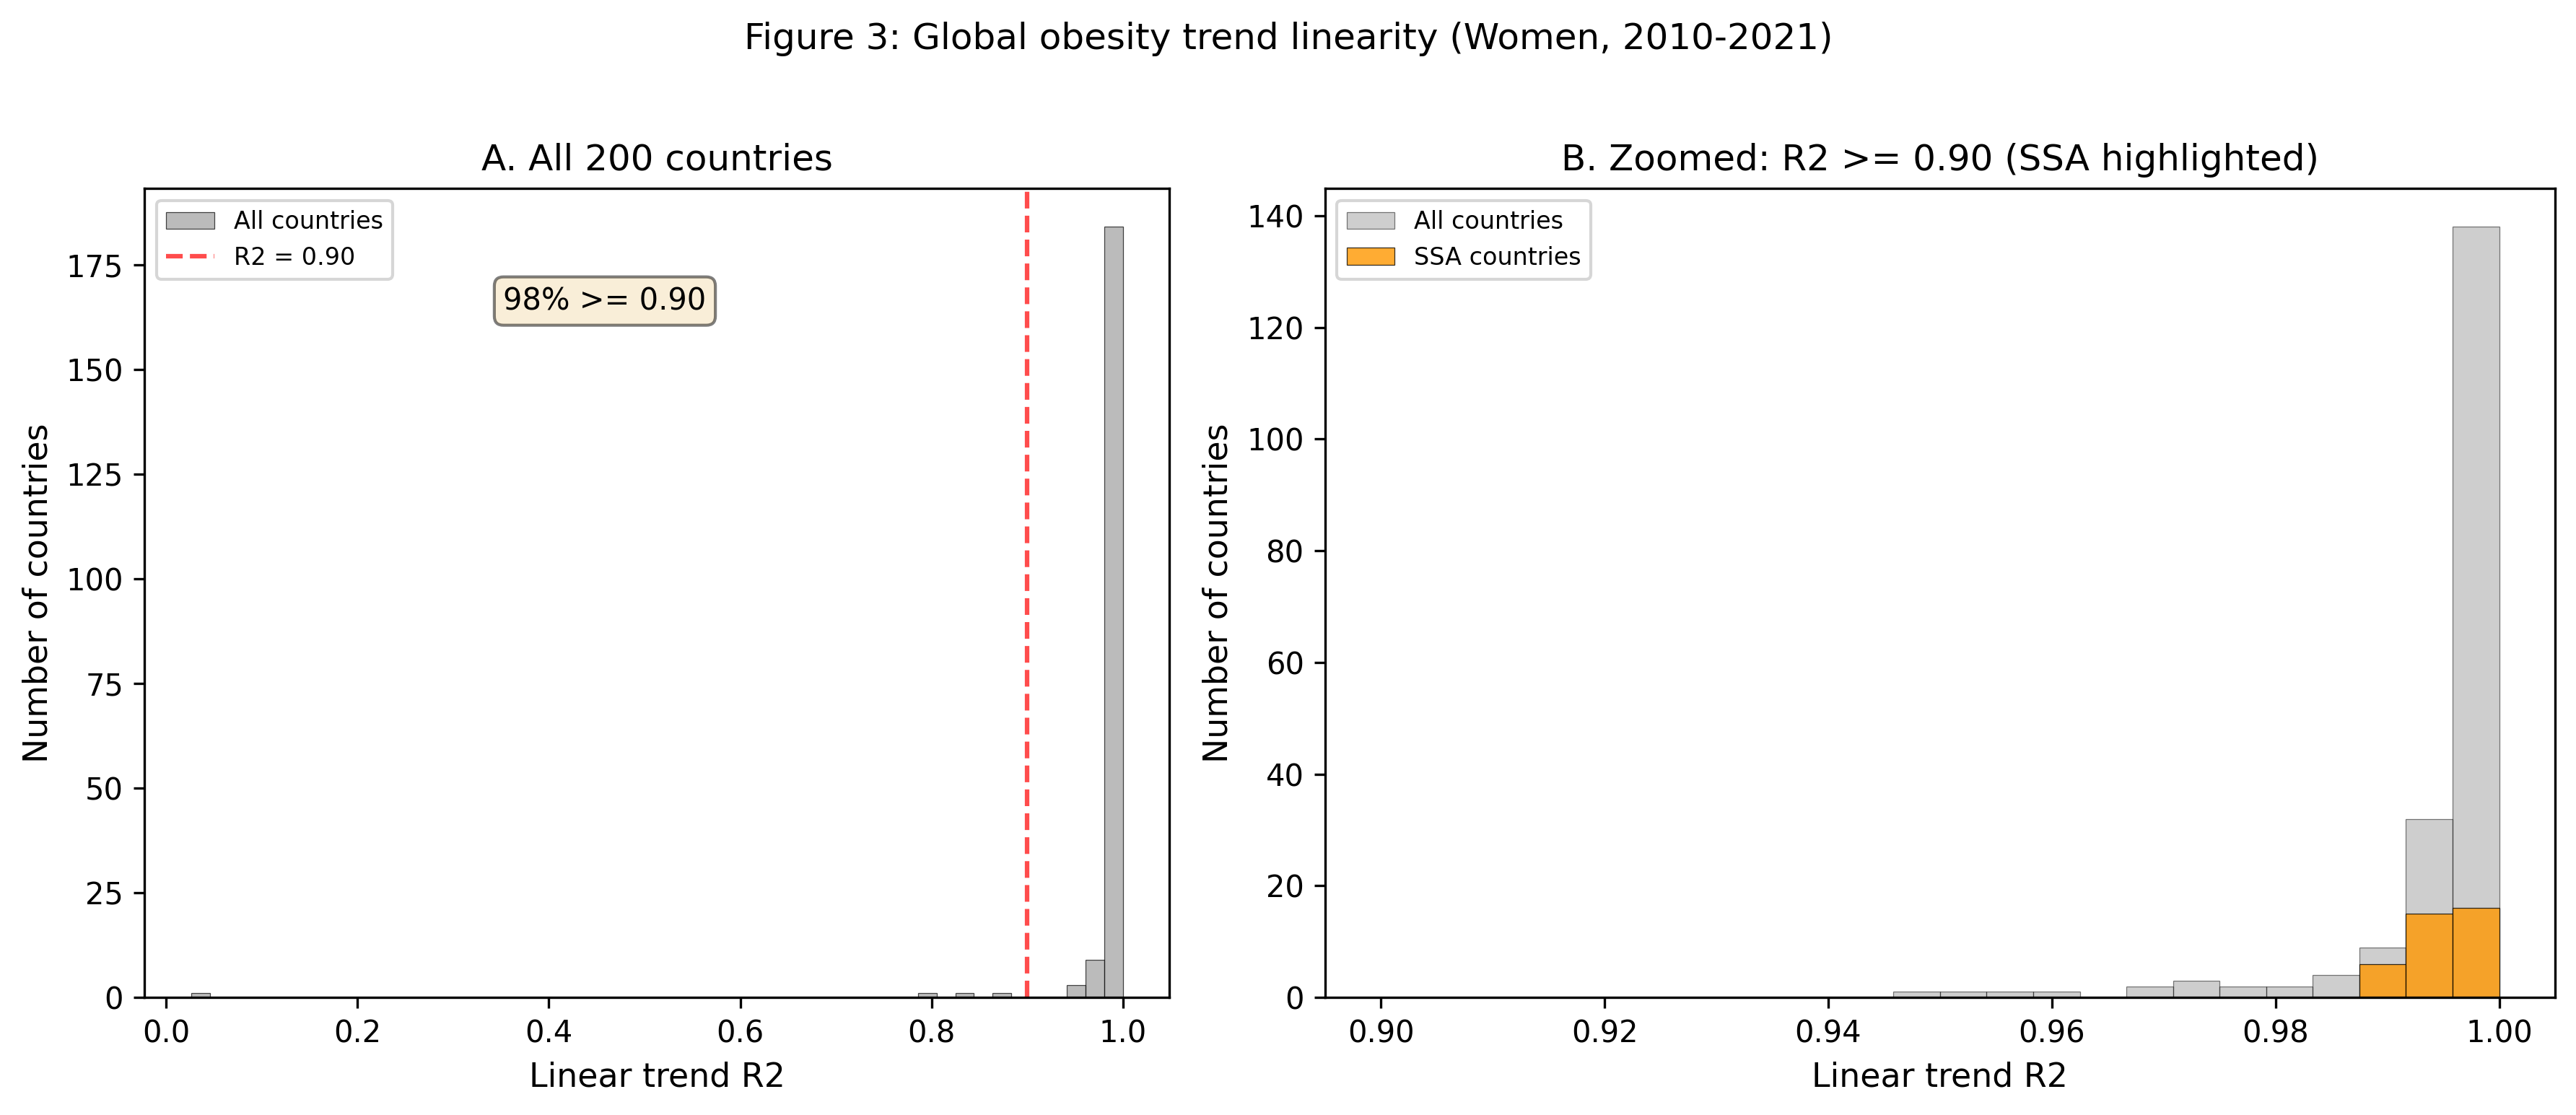
\includegraphics[width=0.7\textwidth]{../../figures/fig3_global_trend_r2.png}
\caption{Distribution of country-specific linear trend $R^2$ for women's obesity, 2010--2021, across 200 countries. 98\% have $R^2 \geq 0.90$, confirming that trend domination is global.}
\label{fig:global_trend}
\end{figure}

This near-universal linearity means that any variable trending upward over the same period will correlate with obesity cross-sectionally, regardless of whether it has a causal relationship. The mechanism generating the sugar paradox in SSA operates worldwide.

\subsection{Implications for Basu et al.\ (2013)}

\citet{basu2013} applied generalized estimating equations to repeated cross-sections in 175 countries and argued that sugar availability independently predicted diabetes prevalence after controlling for income, urbanization, aging, and other food categories. A companion analysis \citep{basu2013ajph} linked soft drink consumption to overweight across 75 countries, a finding cited over 500 times and invoked in WHO guidance on sugar-sweetened beverage taxation \citep{who2023ssb}. That study is not a panel analysis. It uses one observation per country: soft drink consumption averaged over 1997--2007, outcome data from a single year. There is no time dimension, no country fixed effects, no within-country identification. The entire analysis is between-country by design.

Our results show why this matters. Between-country comparisons conflate the effect of sugar with the effect of correlated country-level characteristics---economic development, food system structure, urbanization trajectories---that independently predict obesity and diabetes. Both Basu studies controlled for income and urbanization levels, but level controls do not remove the shared upward trends that drive both sugar availability and obesity over time. The correlated random effects decomposition (Section 3.2) confirms that the entire sugar-obesity association is between-country. The Basu studies measured the development gradient, not a dietary effect.

\subsection{The One-Way Fixed Effects Trap}

Country fixed effects absorb time-invariant between-country differences, but they are not sufficient. Without year fixed effects, the model captures both genuine within-country variation and the shared upward trend common to all countries. \citet{lin2018} illustrate the trap. They regressed average BMI on sugar and processed food imports across 172 countries (1995--2010) with country fixed effects and clustered standard errors but no year fixed effects. They reported a significant positive association ($p < 0.01$), but the coefficient is substantively empty: 0.004 BMI per 10\% increase in sugar imports means a 250\% increase would shift average BMI by 0.1 points. Their specification is exactly the one that captures co-trending: with 172 countries over 16 years, the shared global rise in both BMI and food imports provides statistical power for a spurious signal that year fixed effects would absorb.

The soybean oil case study (Section 4.4) shows this trap in our data. Soybean oil is significant under one-way country FE ($t_{\text{cl}} = 2.09$) but null under two-way FE ($t_{\text{cl}} = 0.70$). The co-trending signal that disappears when year effects are absorbed is exactly the signal that one-way FE captures.

In our SSA data, sugar is null under every within-country specification, including the most generous: non-clustered standard errors, one-way country fixed effects, no additional controls ($t = 0.66$, $p = 0.51$). Even this maximally favorable specification yields a null result. There is nothing for year effects to absorb because the sugar-obesity association is entirely between-country.

The combination of one-way FE and non-clustered standard errors compounds the problem. Clustering inflates standard errors by 2.6$\times$ to 2.9$\times$ for sugar specifications in our data \citep{bertrand2004, abadie2023}. Effects that appear significant with non-clustered errors in a country-level panel may not survive appropriate clustering.

\subsection{The GDP Positive Control}

To confirm that our methodology can detect real within-country associations, we apply the same specification cascade to GDP per capita. GDP correlates positively with obesity cross-sectionally ($r = 0.73$, $p < 0.001$). Under two-way fixed effects, the coefficient is null ($t_{\text{cl}} = -0.28$). Under entity-specific detrending, GDP is significantly negative: $\hat{\beta} = -1.10$, $t_{\text{cl}} = -4.12$.

The sign reversal is meaningful. Cross-sectionally, richer countries have higher obesity. Within countries, after removing each country's linear trend, years of faster GDP growth correspond to slightly slower obesity growth. This detrended relationship is the only food or economic variable to achieve significance in our panel ($t = -4.12$). It confirms two things: the methodology has power to detect within-country associations when they exist, and the null for food supply variables is not a power artifact.

\begin{figure}[htbp]
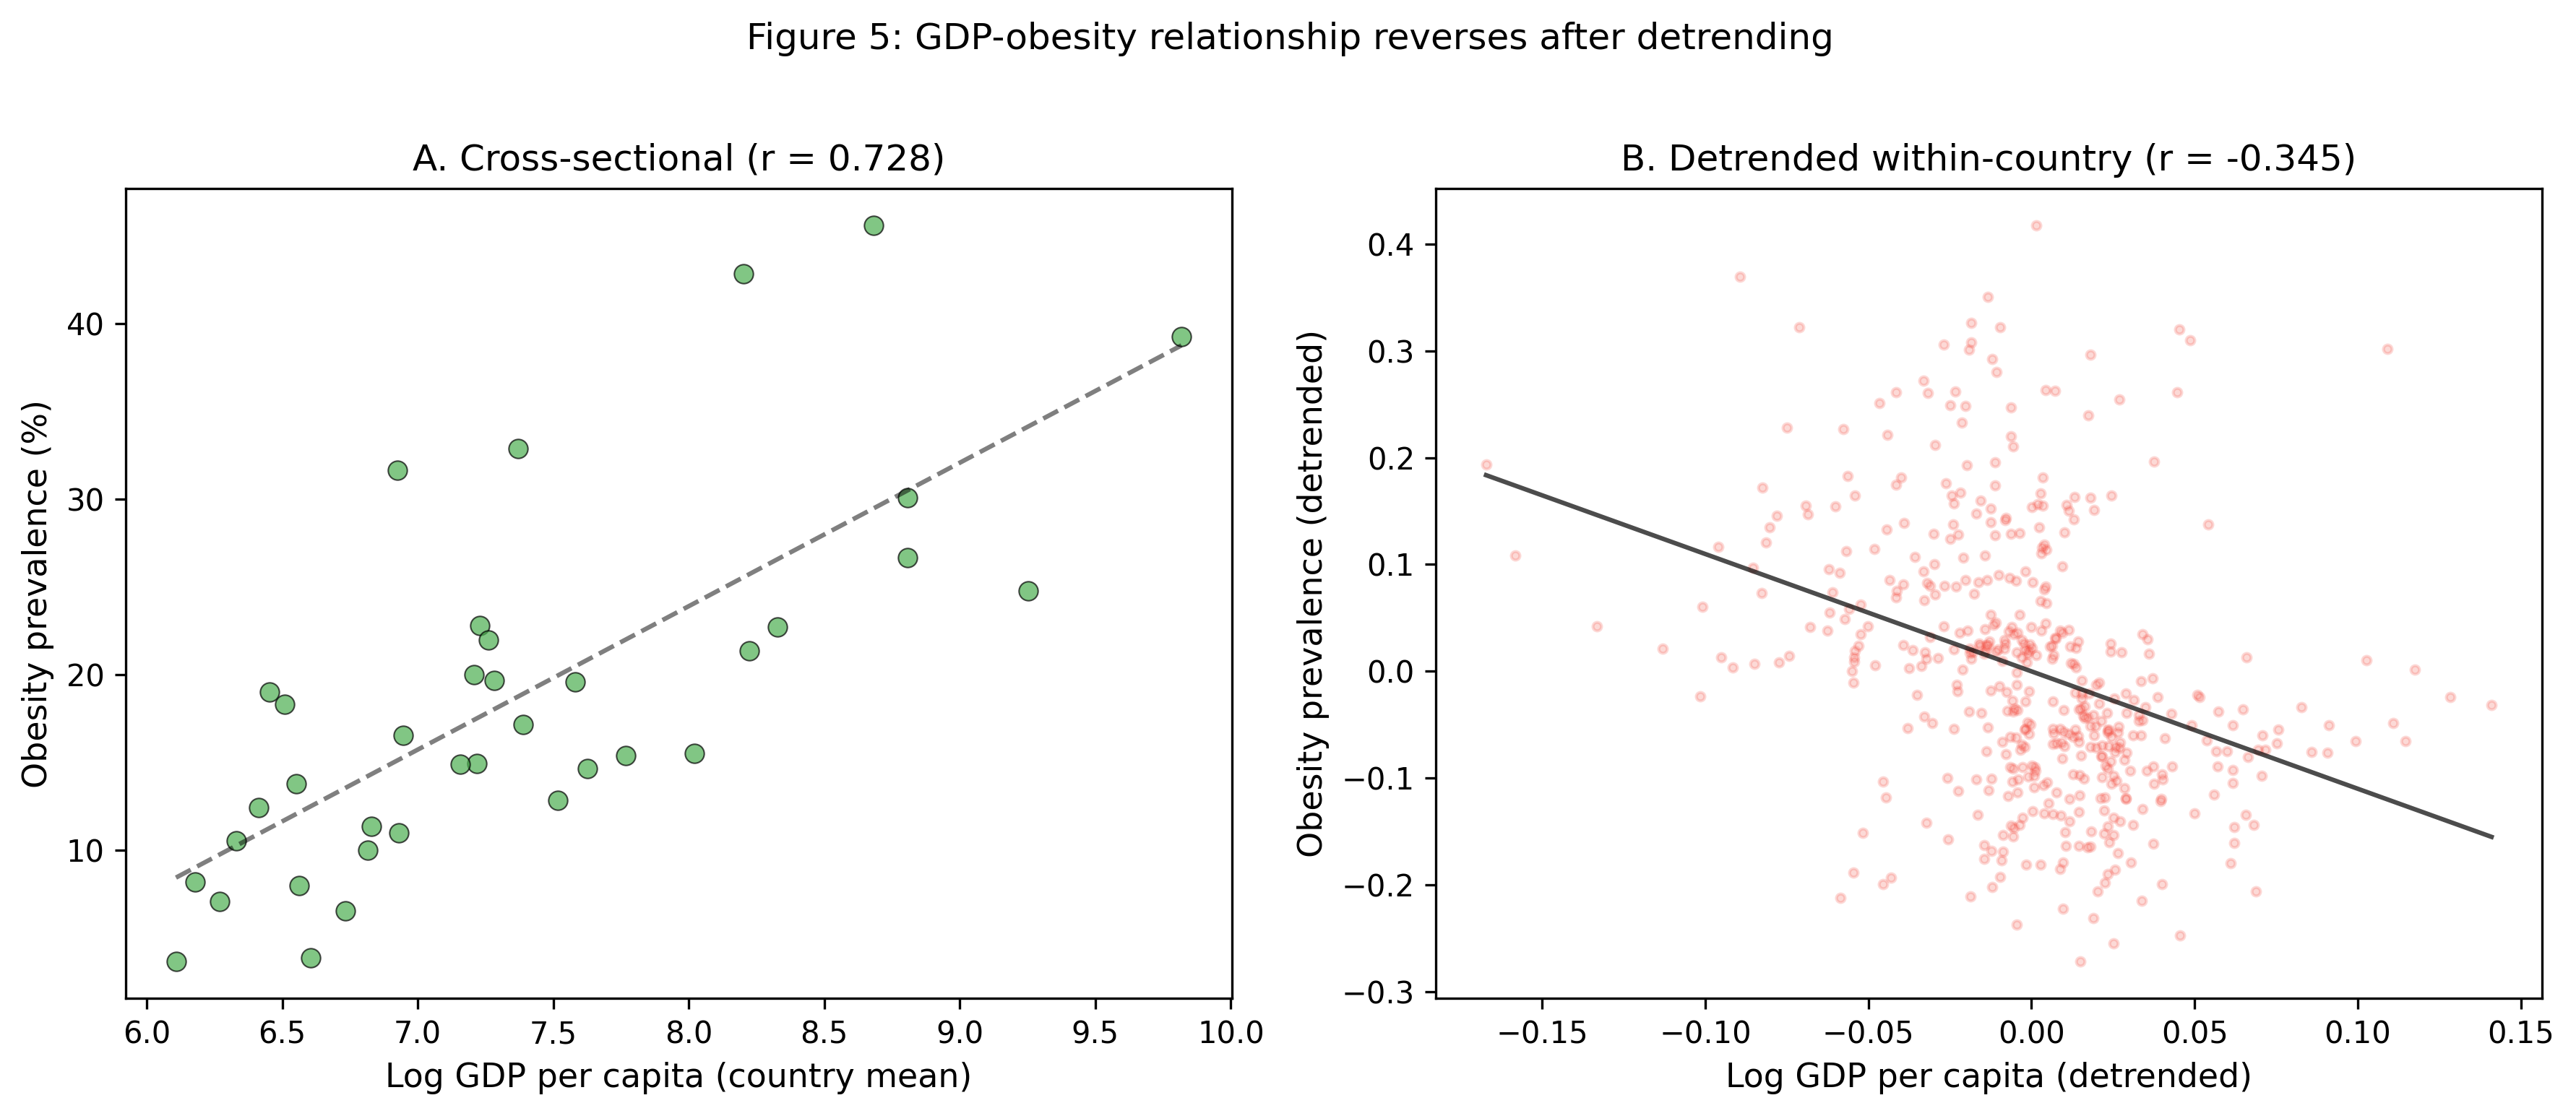
\includegraphics[width=\textwidth]{../../figures/fig5_gdp_control.png}
\caption{GDP per capita as positive control. Cross-sectional: $r = 0.73$ (positive). Detrended: $r = -0.35$, $t_{\text{cl}} = -4.12$ (negative). The sign reversal confirms the method detects real within-country associations. Sugar and the FAOSTAT food-group variables show no comparable signal.}
\label{fig:gdp_control}
\end{figure}

% -----------------------------------------------
% 6. What Predicts Cross-Country Obesity Change
% -----------------------------------------------
\section{What Predicts Cross-Country Obesity Change}

If food supply changes do not predict obesity change, what does? We regress the 2010--2020 change in women's obesity on corresponding changes in urbanization, sugar supply, vegetable oil supply, and GDP per capita, plus initial (2010) obesity prevalence. The regression uses one observation per country ($N = 37$).

Table~\ref{tab:change} reports the results. The model explains 41\% of the variance in obesity change ($R^2 = 0.405$). Of the five predictors, only initial obesity is significant: $\hat{\beta} = 0.12$ ($t = 3.45$, $p = 0.002$). Countries with higher obesity in 2010 gained more obesity over the following decade. Sugar change contributes nothing ($t = -0.22$). GDP change contributes nothing ($t = 0.46$). Urbanization change is marginally positive ($t = 1.73$, $p = 0.09$). Vegetable oil change is marginally negative ($t = -1.84$, $p = 0.08$), though this marginal result does not survive more demanding specifications.

\begin{table}[htbp]
\caption{Cross-country change regression, 2010--2020. Dependent variable: change in women's obesity prevalence (percentage points). $N = 37$ countries. $R^2 = 0.405$.}
\label{tab:change}
\begin{tabular*}{\textwidth}{@{\extracolsep\fill}lrrr}
\toprule
Predictor & $\hat{\beta}$ & $t$ & $p$ \\
\midrule
$\Delta$ Urbanization & 0.154 & 1.73 & 0.094 \\
$\Delta$ Sugar supply & $-0.002$ & $-0.22$ & 0.830 \\
$\Delta$ Vegetable oils & $-0.008$ & $-1.84$ & 0.075 \\
$\Delta$ GDP per capita & 0.770 & 0.46 & 0.652 \\
Initial obesity (2010) & 0.120 & 3.45 & 0.002 \\
\bottomrule
\end{tabular*}
\end{table}

All 37 countries gained obesity over this period. The mean gain was 4.9 percentage points; the range was 1.4 to 9.4. The pattern is divergence, not convergence: countries with higher initial obesity gained more, not less. A country starting at 25\% obesity in 2010 gained roughly 1.8 percentage points more than a country starting at 10\%.

This divergence explains why cross-sectional correlations between food supply and obesity grow stronger over time. High-sugar countries tend to be the same high-obesity countries, and these countries gain obesity faster than low-obesity countries. The gap widens year by year, strengthening the cross-sectional association at any point in time. But the widening is driven by initial conditions, not by sugar supply changes. Food supply variables add nothing to the prediction of obesity change once initial obesity is included.

The divergence pattern is consistent with structural determinants: built environment, food retail infrastructure, sedentary employment share, and other features of economic development that correlate with initial obesity levels. These structural conditions are self-reinforcing. Countries further along the economic transition have environments that promote weight gain, and these environments accumulate rather than dissipate. The implication is that cross-country obesity differences reflect development trajectories, not the composition of national food supply.

% -----------------------------------------------
% 7. Discussion
% -----------------------------------------------
\section{Discussion}

\subsection{What the Paradox Means for Sugar Tax Evidence}

Sugar-sweetened beverage taxes have been implemented or proposed in over 40 countries \citep{who2023ssb}, drawing in part on cross-sectional evidence linking sugar availability to metabolic disease \citep{basu2013, basu2013ajph}. Our findings do not imply that sugar is harmless. Individual-level prospective cohorts and meta-analyses consistently link sugar-sweetened beverage consumption to type 2 diabetes and metabolic syndrome \citep{imamura2015, malik2010}, and a recent global analysis attributed 2.2 million new diabetes cases to these beverages \citep{laracastor2025}. What we show is that national food supply data cannot distinguish the effect of sugar from the effect of correlated development trends. Policy arguments built on cross-country food supply associations rest on weaker identification than commonly assumed.

South Africa's sugar-sweetened beverage tax, implemented in April 2018, illustrates the difficulty. South Africa's NCD-RisC obesity trajectory shows no deflection after 2018, continuing its pre-tax linear trend. But the NCD-RisC smoothing model imposes temporal continuity by design, so the absence of a visible break cannot be taken as evidence that the tax had no effect. The data most commonly used to study national-level food-obesity relationships cannot resolve the kind of sharp policy discontinuity that would provide clean within-country identification. Evaluating SSB taxes requires survey data collected before and after implementation \citep{colchero2016}, not modeled trajectories that smooth over exactly the variation researchers need.

\subsection{What the Paradox Means for Dietary Risk Assessment}

The Global Burden of Disease study estimates diet-attributable deaths using intake data that faces the same structural problem \citep{gbd2019}. GBD dietary risk estimates combine survey data with food supply proxies and model-based extrapolation. To the extent that these estimates rely on cross-country variation in food supply to calibrate risk, they inherit the confounding structure we document. Risk attributed to specific food categories based on national supply data should be interpreted with caution.

The failure of food supply data to predict within-country obesity also says something about FAOSTAT as a health research instrument. Food Balance Sheets measure national availability at the supply level: production plus imports minus exports minus non-food uses, divided by population. They do not capture distribution within countries, food waste, processing, or actual dietary intake. \citet{delgobbo2015} compared FAO supply estimates to individual-level dietary surveys across 113 countries and found that FAO data overestimates intake by 50--270\% for most food groups. \citet{vonderschmidt2024} showed that FAOSTAT's 2014 methodology revision creates discontinuities that can reverse apparent trends in food supply series, a problem for any study combining pre- and post-revision data. The gap between supply-level availability and individual consumption may be large enough to obscure genuine diet-disease relationships, even if such relationships exist at the individual level. Recent FAOSTAT-based studies extend the same design to total energy and nutritive-value supplies \citep{siminiuc2025,delgadopertinez2026}; our comparator shows that aggregate energy and macronutrient totals do not escape the trend problem in SSA. Cross-national ecological studies using other food classification systems face the same problem: \citet{monteiro2018} found that ultra-processed food availability predicted obesity across 19 European countries, a design that cannot separate co-trending from causation. This is not a reason to discard FAOSTAT data for health research. It is a reason to be precise about what cross-national food supply comparisons can and cannot identify.

\subsection{Better Identification Strategies}

If cross-sectional and one-way fixed-effects designs are inadequate, three approaches might provide stronger evidence.

First, policy discontinuities. Sugar taxes, trade liberalization events, or agricultural policy changes create sharp temporal variation in specific food categories. Difference-in-differences or synthetic control designs exploiting these events could provide within-country identification that panel fixed effects cannot.

Second, subnational data. District- or province-level panels increase the number of units and the variation in food environments while holding national-level trends constant. Subnational data also allows analysis of food retail access, supermarket penetration, and ultra-processed food availability, measures closer to dietary exposure than national supply totals.

Third, individual-level longitudinal surveys. Panel studies tracking dietary intake and health outcomes eliminate the ecological fallacy inherent in country-level analysis. Such data exist for some high-income countries but remain largely absent in Sub-Saharan Africa.

\subsection{Limitations}

Four limitations bear on interpretation. First, the panel covers 37 of 48 SSA countries; 11 are absent from the comparable FAOSTAT release. Second, NCD-RisC smoothing compresses within-country variation, working against detecting within-country associations. The consistency of the null across six specifications, including long differences that compare only decade endpoints, argues this is not the sole explanation. Third, we analyze food supply, not food intake. The paradox could reflect a failure of FAOSTAT to capture dietary variation rather than a genuine absence of diet-obesity relationships. Fourth, our panel period (2010--2022) is short enough that slow-acting dietary effects could be missed by trend-removal methods.

\subsection{Reframing the Question}

The field should shift its question. Instead of asking which food causes obesity at the population level, using data that cannot answer that question, researchers should ask what structural conditions drive divergent obesity trajectories across countries. Our evidence points to initial conditions and development pathways rather than dietary composition as the primary source of cross-country variation.

This is not simply the ecological fallacy by another name. \citet{robinson1950} warned that group-level associations may not hold for individuals. The ``Australian Paradox'' \citep{barclay2011} showed that sugar intake and obesity can diverge within a single country over time. We show something more specific than either: a quantifiable mechanism that makes an entire class of study designs unreliable, regardless of the food variable, the region, or the analytical refinement applied. Trend domination absorbs 99.4\% of outcome variance. The soybean oil case study shows that standard robustness tests---clustered standard errors, leave-one-out exclusion, Oster bounds---cannot distinguish co-trending from causation. The problem is global, affecting 98\% of countries.

The field built a large evidence base from cross-national food supply associations. That evidence base cannot answer the question it was designed to answer. The question now is not which food causes obesity at the population level, but what structural conditions drive the divergent trajectories along which countries are gaining weight. Our evidence points to initial conditions and development pathways. The data needed to go further---subnational panels, individual-level longitudinal surveys, policy discontinuity designs---exist in fragments but not yet at the scale required. Until they do, cross-sectional food supply studies will continue to find strong associations that reflect shared trends rather than dietary effects.

% -----------------------------------------------
% Data and Code Availability
% -----------------------------------------------
\section*{Data and Code Availability}

All data and code required to reproduce the analyses in this paper are publicly available at \url{https://github.com/mamboanye/sugar-paradox}.

\bibliography{references}

\end{document}
